\chapter{Результаты решения задачи 3D локализации}

\section{Используемые данные}

В качестве датасет использовался не LIDC-IDRI непосредственно, как это было сделано в решении задачи 2d-сегментации, а его подможество LUNA, содержащее 888 сканов, где на каждом скане присутствует одна размеченная опухоль. Метка представлена в виде bounding box.

\section{Детали реализации}

\subsection{Реализация DeepSEED}

В оригинальной работе было предложено подавать на вход сети обрезанные участки КТ изображений размера $128^3$, однако такая размерность входных данный требует вычислительных ресурсов, которые были недоступны во время реализации, что привело к уменьшению размерности входа до $64^3$.

\subsection{Реализация CGAN}

Бейслайн архитектура CGAN, формат и размерность входных и выходных данных была полностью заимствованы у авторов статьи.

Во время обучения была обнаружена следующая проблема: лосс дискриминатора уменьшался гораздо лучше, чем лосс генератора, и начиная с некоторой эпохи дискриминатор почти всегда отличал генерированные изображения от оригинальных.

\subsection{Реализация Адаптивной нормализации}

Адаптивная нормализация была добавлена в сеть вместо батчевой нормализации. Она применяется после всех блоков (свертка, активация) и в кодировщике, и в декодировщике кроме первого слоя. В качестве входа $x$ формулы \eqref{eq:adain} используется тензор, полученный на выходе активации, а в качестве параметра $y$ используется выход побочной сети, имеющей простую архитектуру - 3 полносвязных слоя, причем первые два разделены между всеми побочными сетями. Данная архитектура позволяет выявить эффективные параметры афинного преобразования посредством обучения.

\section{Результаты}

\subsection{Результаты локализации с помощью DeepSEED}

В качестве метрик качества были выбраны ROC и FROC кривые. Стоит отметить, что FROC-анализ является достаточно популярным в области локализации новообразований легких. FROC-кривая аналогична ROC-кривой, но по оси $x$ отмечен не процент ложно положительных результатов, а среднее количество ложно-положительных bounding-box-ов на один скан.

Для визуализации результатов на рисунках \ref{roc-baseline} и \ref{froc-baseline} предоставлены графики, полученные в результате тестирования обученной модели.

\begin{figure}[!h]
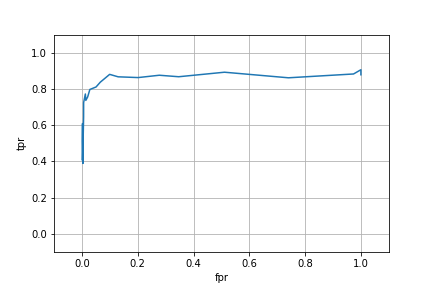
\includegraphics[width=\linewidth]{roc.png}
\caption{ROC результаты}\label{roc-baseline}
\centering
\end{figure}

\begin{figure}[!h]
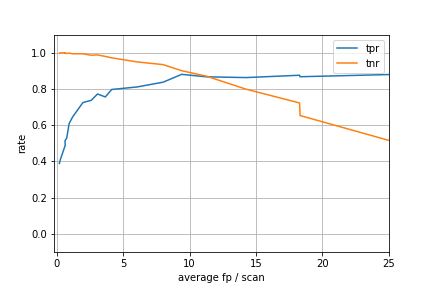
\includegraphics[width=\linewidth]{froc.png}
\caption{FROC результаты}\label{froc-baseline}
\centering
\end{figure}

Интересно также сравнить FROC кривые полученные нами и авторами оригинальной статьи. На рисунке \ref{froc-lifan} приведена FROC-кривая из оригинальной статьи.

\begin{figure}[!h]
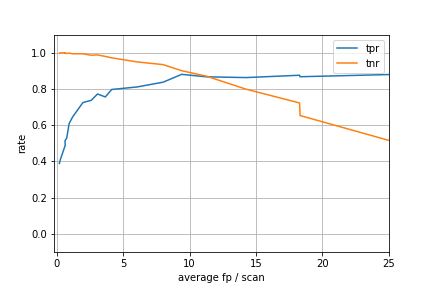
\includegraphics[width=\linewidth]{froc.png}
\caption{FROC-результаты (Li, Fan)}\label{froc-lifan}
\centering
\end{figure}

Стоит отметить схожесть кривых. Полученные результаты оказались несколько хуже результатов в статье, что возможно объяснить вынужденным сокращением размерностей обрезанных изображений, подаваемых на вход DeepSEED.

\subsection{Результаты обучения CGAN}

Для оценки качеcтва работы сети CGAN в первую очередь применялся визуальный анализ. На рисунке \ref{mirskiy-results} представлены примеры генерированных изображений, заимствованные из работы Мирского и др. На рисунке \ref{cgan-baseline-results} представлены результаты работы CGAN, предложенной в статье, но обученной нами. На рисунке \ref{cgan-adain-results} представлены результаты работы CGAN, в архитектуру которого вместо BN добавлен AdaIN

\begin{figure}[!h]
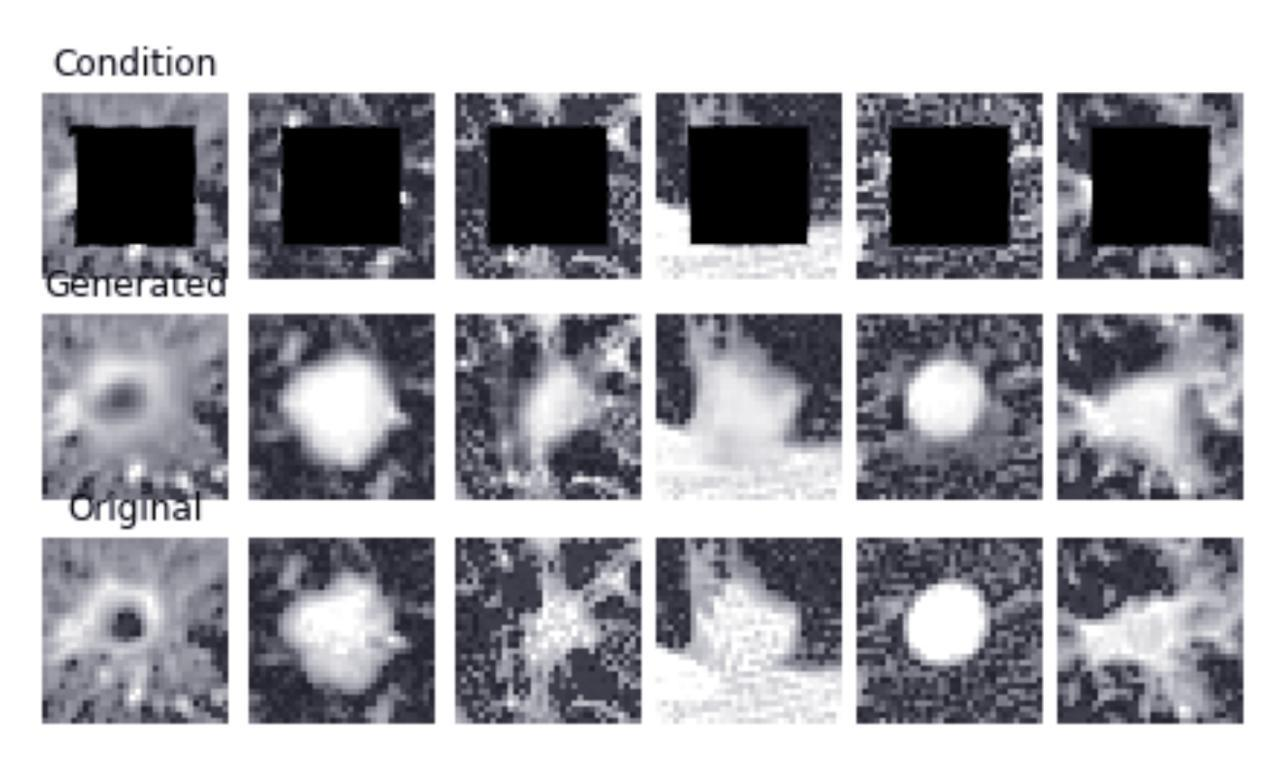
\includegraphics[width=\linewidth]{mirskiy-results.jpg}
\caption{Пример генерированных изображений (Mirsky et.al.)}\label{mirskiy-results}
\centering
\end{figure}

\begin{figure}[!h]
\includegraphics[width=\linewidth]{}
\caption{Пример генерированных изображений (Без AdaIN)}\label{cgan-baseline-results}
\centering
\end{figure}

\begin{figure}[!h]
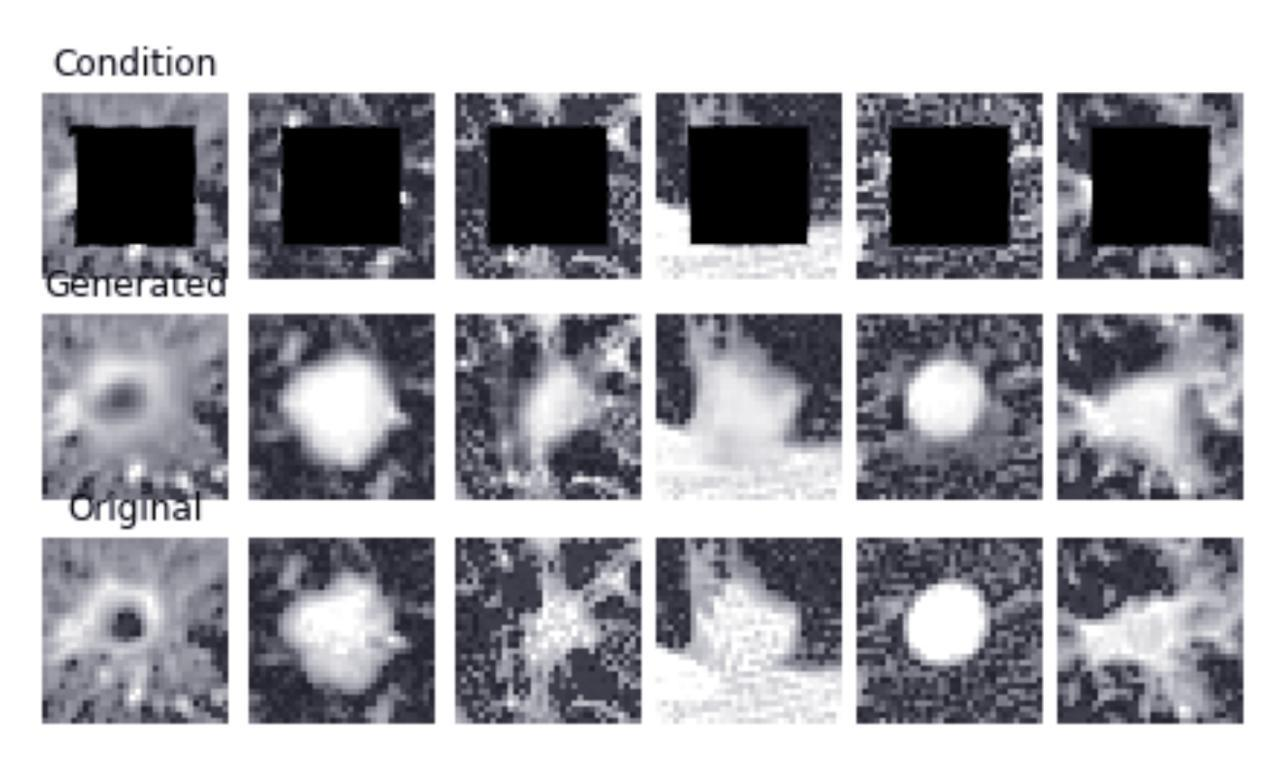
\includegraphics[width=\linewidth]{mirskiy-results.jpg}
\caption{Пример генерированных изображений (С использованием AdaIN)}\label{cgan-adain-results}
\centering
\end{figure}